\documentclass[12pt, a4paper]{article}

% -------------------------------------------------------------------------
% Packages
% -------------------------------------------------------------------------
\usepackage[margin=2.5cm, headheight=15pt]{geometry}
\usepackage{booktabs}
\usepackage{tabularx}
\usepackage{array}
\usepackage{longtable}
\usepackage{xcolor}
\usepackage{titlesec}
\usepackage{parskip}
\usepackage{hyperref}
\usepackage{enumitem}
\usepackage{fancyhdr}
\usepackage{colortbl}
\usepackage[T1]{fontenc}
\usepackage{lmodern}
\usepackage{tikz}
\usetikzlibrary{positioning}
\usepackage{mdframed}
\usepackage{tcolorbox}
\tcbuselibrary{listings}
\usepackage{listings}
\usepackage{calc}

% -------------------------------------------------------------------------
% Colors
% -------------------------------------------------------------------------
\definecolor{pollityblue}{RGB}{0, 84, 166}
\definecolor{pollitylightblue}{RGB}{220, 235, 252}
\definecolor{phase0color}{RGB}{100, 100, 100}
\definecolor{phase1color}{RGB}{0, 128, 0}
\definecolor{phase2color}{RGB}{200, 120, 0}
\definecolor{phase3color}{RGB}{166, 0, 0}
\definecolor{lightgray}{RGB}{248, 248, 248}
\definecolor{midgray}{RGB}{180, 180, 180}
\definecolor{codebg}{RGB}{240, 240, 240}
\definecolor{arrowcolor}{RGB}{0, 84, 166}

% -------------------------------------------------------------------------
% Section formatting
% -------------------------------------------------------------------------
\titleformat{\section}{\large\bfseries\color{pollityblue}}{}{0em}{}[\titlerule]
\titleformat{\subsection}{\normalsize\bfseries\color{pollityblue!80!black}}{}{0em}{\thesubsection\quad}
\titleformat{\subsubsection}{\normalsize\bfseries}{}{0em}{}

\renewcommand{\thesubsection}{\arabic{subsection}}

% -------------------------------------------------------------------------
% Header / Footer
% -------------------------------------------------------------------------
\pagestyle{fancy}
\fancyhf{}
\fancyhead[L]{\small\textit{Pollity --- MVP Plan \& Architecture}}
\fancyhead[R]{\small\textit{Internal / Confidential}}
\fancyfoot[C]{\thepage}
\renewcommand{\headrulewidth}{0.4pt}

% -------------------------------------------------------------------------
% Hyperref
% -------------------------------------------------------------------------
\hypersetup{
    colorlinks=true,
    linkcolor=pollityblue,
    urlcolor=pollityblue,
    pdftitle={Pollity MVP Plan},
    pdfauthor={Piyush Zaware}
}

% -------------------------------------------------------------------------
% Custom boxes
% -------------------------------------------------------------------------
\tcbuselibrary{skins, breakable, listings}

\newtcolorbox{thesisbox}{
    colback=pollitylightblue,
    colframe=pollityblue,
    boxrule=1.5pt,
    arc=4pt,
    left=8pt, right=8pt, top=6pt, bottom=6pt,
    fonttitle=\bfseries\color{pollityblue},
    title=Core Thesis
}

\newtcolorbox{phasebox}[2]{
    colback=#1!8!white,
    colframe=#1,
    boxrule=1pt,
    arc=4pt,
    left=8pt, right=8pt, top=6pt, bottom=6pt,
    fonttitle=\bfseries\color{#1},
    title=#2,
    breakable
}

\newtcblisting{treebox}{
    colback=codebg,
    colframe=midgray,
    boxrule=0.5pt,
    arc=2pt,
    left=8pt, right=8pt, top=6pt, bottom=6pt,
    listing only,
    listing options={
        basicstyle=\ttfamily\small,
        breaklines=true,
        columns=fullflexible,
        keepspaces=true
    },
    breakable
}

% -------------------------------------------------------------------------
% Code/tree style
% -------------------------------------------------------------------------
\lstset{
    basicstyle=\ttfamily\small,
    backgroundcolor=\color{codebg},
    frame=single,
    framerule=0.5pt,
    rulecolor=\color{midgray},
    breaklines=true,
    columns=fullflexible,
    keepspaces=true,
    showstringspaces=false
}

% -------------------------------------------------------------------------
\begin{document}

% =========================================================================
% TITLE PAGE
% =========================================================================
\begin{titlepage}
    \centering
    \vspace*{1.5cm}

    {\color{pollityblue}\rule{\linewidth}{2pt}}\\[0.4cm]
    {\Huge\bfseries\color{pollityblue} POLLITY}\\[0.3cm]
    {\large\itshape Building India's Last Mile of Digital Governance}\\[0.2cm]
    {\color{pollityblue}\rule{\linewidth}{2pt}}\\[1.2cm]

    {\LARGE\bfseries MVP Plan \& Architecture}\\[0.4cm]
    {\large Jan-Sunwai: Phase 0 to Beta Launch}\\[1.2cm]

    \begin{tabular}{ll}
        \textbf{Version:}         & 1.0 \\[0.3em]
        \textbf{Prepared by:}     & Piyush Zaware, Co-Founder \& CTO \\[0.3em]
        \textbf{Date:}            & March 2026 \\[0.3em]
        \textbf{Build Target:}    & Q3--Q4 2026 Beta Launch \\[0.3em]
        \textbf{Beta Goal:}       & 50 active users, NPS $>$ 40 \\[0.3em]
        \textbf{MVP Scope:}       & Jan-Sunwai (grievance management only) \\
    \end{tabular}

    \vspace{1.5cm}

    \begin{thesisbox}
        Build one thing well: \textbf{Jan-Sunwai}. A WhatsApp-first grievance intake and case
        management system for representative offices. Nothing else until 50 users are
        active and NPS $>$ 40. Each additional agent (Vidhayak-Mitra, Vikas-Tracker,
        Nagrik-Setu) is roadmap --- not MVP.
    \end{thesisbox}

    \vfill

    {\color{midgray}\rule{0.5\linewidth}{0.5pt}}\\[0.3cm]
    {\small pollity.in \quad $\cdot$ \quad hello@pollity.in}\\
    {\small\textcopyright\ 2026 Pollity. Confidential.}
\end{titlepage}

% =========================================================================
% TABLE OF CONTENTS
% =========================================================================
\tableofcontents
\newpage

% =========================================================================
% SECTION 1: TECH STACK
% =========================================================================
\section{Technology Stack}

Every choice below is made with three constraints in mind: (1) plays to the founding team's existing skills, (2) keeps costs near-zero during pre-seed, and (3) keeps data in India for DPDP Act compliance.

\begin{table}[ht]
\centering
\caption{Full Technology Stack}
\renewcommand{\arraystretch}{1.4}
\begin{tabularx}{\textwidth}{>{\bfseries}p{2.8cm} p{4.2cm} X}
\toprule
\rowcolor{pollitylightblue}
\textbf{Layer} & \textbf{Choice} & \textbf{Reason} \\
\midrule
Backend        & Python + FastAPI         & Plays to CTO strengths; async-ready; native ML library support \\
\midrule
Frontend       & Next.js 14 (TypeScript)  & App Router + server components; excellent for data dashboards; large contractor ecosystem \\
\midrule
Database       & PostgreSQL via Supabase  & Multi-tenant row-level security; managed Postgres; free tier for development; built-in auth \\
\midrule
Cache / Queue  & Redis                    & WhatsApp webhook message queue; rate limiting; fast session store \\
\midrule
WhatsApp       & Meta Business API        & Direct webhook integration; no middleware cost; official channel for citizen communication \\
\midrule
NLP / AI       & Claude API (Anthropic)   & Best-in-class multilingual understanding; handles Hinglish, Hindi, Marathi; context-aware classification \\
\midrule
Auth           & Supabase Auth            & Row-level security built into Postgres; free tier; JWT-based; easy multi-tenant isolation \\
\midrule
Hosting        & AWS Mumbai (ap-south-1)  & DPDP Act compliance --- all citizen data must reside in India; lowest latency for Indian users \\
\midrule
CI/CD          & GitHub Actions           & Free; native integration with repo; deploy on merge to main \\
\midrule
Containers     & Docker + Docker Compose  & Dev/prod parity; enables contractor onboarding without environment setup friction \\
\midrule
Monitoring     & Sentry + PostHog         & Sentry: error tracking + alerts; PostHog: product analytics, NPS, session recording \\
\bottomrule
\end{tabularx}
\end{table}

\newpage

% =========================================================================
% SECTION 2: MVP SCOPE
% =========================================================================
\section{MVP Scope: Jan-Sunwai v1}

\subsection{What Jan-Sunwai Does}

Jan-Sunwai is a WhatsApp-first grievance intake and case management system. The citizen never needs to open a website. The representative's office manages everything through a web dashboard.

\vspace{0.5em}

\begin{center}
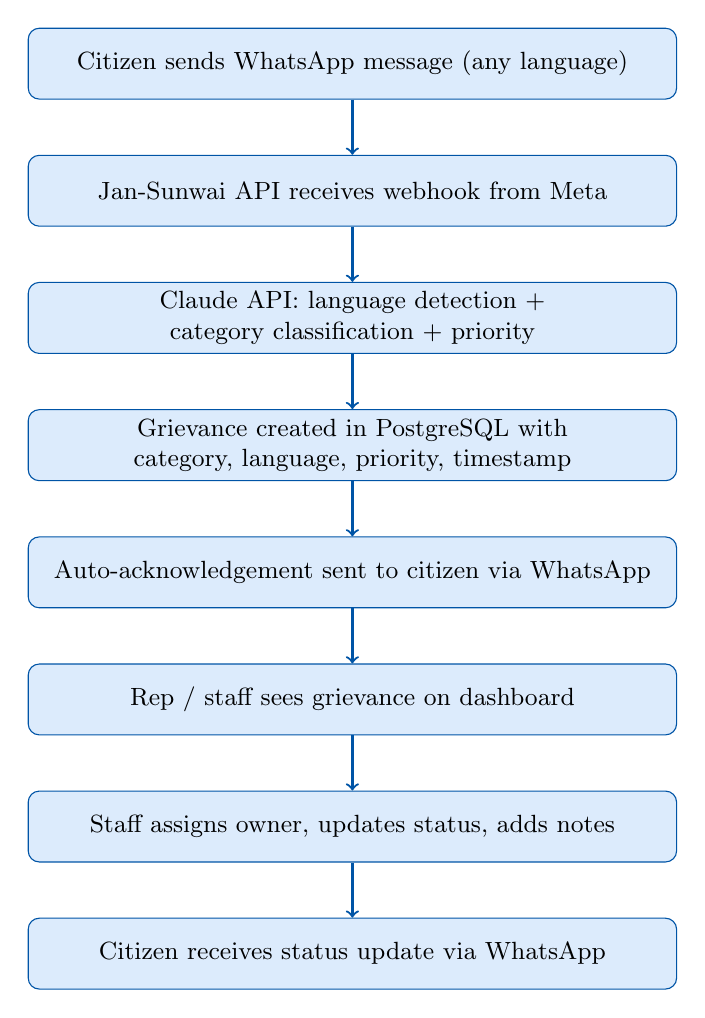
\begin{tikzpicture}[
    node distance=0.7cm,
    box/.style={
        rectangle, rounded corners=4pt,
        draw=pollityblue, fill=pollitylightblue,
        text width=8cm, align=center,
        minimum height=0.9cm, font=\small
    },
    arrow/.style={->, thick, color=pollityblue}
]
    \node[box] (n1) {Citizen sends WhatsApp message (any language)};
    \node[box, below=of n1] (n2) {Jan-Sunwai API receives webhook from Meta};
    \node[box, below=of n2] (n3) {Claude API: language detection + category classification + priority};
    \node[box, below=of n3] (n4) {Grievance created in PostgreSQL with category, language, priority, timestamp};
    \node[box, below=of n4] (n5) {Auto-acknowledgement sent to citizen via WhatsApp};
    \node[box, below=of n5] (n6) {Rep / staff sees grievance on dashboard};
    \node[box, below=of n6] (n7) {Staff assigns owner, updates status, adds notes};
    \node[box, below=of n7] (n8) {Citizen receives status update via WhatsApp};

    \draw[arrow] (n1) -- (n2);
    \draw[arrow] (n2) -- (n3);
    \draw[arrow] (n3) -- (n4);
    \draw[arrow] (n4) -- (n5);
    \draw[arrow] (n5) -- (n6);
    \draw[arrow] (n6) -- (n7);
    \draw[arrow] (n7) -- (n8);
\end{tikzpicture}
\end{center}

\subsection{What Jan-Sunwai Does NOT Do in v1}

The following are explicitly out of scope for the MVP. Each item below is a future roadmap feature, not a v1 deliverable.

\begin{itemize}[leftmargin=1.5em, itemsep=0.2em]
    \item CPGRAMS integration (requires 12--36 month government MOU negotiation)
    \item Vidhayak-Mitra: legislative research agent
    \item Vikas-Tracker: MPLADS/MLALADS fund management agent
    \item Nagrik-Setu: social media and constituency engagement agent
    \item Voice/IVR call intake
    \item SMS intake
    \item Fund tracking or budget analysis
    \item Social media monitoring or publishing
    \item Parliamentary procedure support
\end{itemize}

\subsection{Grievance Categories (v1 NLP Taxonomy)}

The Claude API classifier will map incoming grievances to 8 top-level categories, each with sub-categories to be refined during beta:

\begin{table}[ht]
\centering
\caption{Jan-Sunwai v1 Grievance Taxonomy}
\renewcommand{\arraystretch}{1.3}
\begin{tabularx}{\textwidth}{>{\bfseries}p{3cm} X}
\toprule
\rowcolor{pollitylightblue}
\textbf{Category} & \textbf{Examples} \\
\midrule
Roads \& Infrastructure & Pothole, streetlight, broken footpath, drainage \\
Water \& Sanitation     & Water supply, sewage, open defecation, cleaning \\
Electricity             & Power outage, billing dispute, new connection \\
Health                  & Hospital access, medicine availability, ASHA worker \\
Education               & School building, teacher absence, mid-day meal \\
Housing \& Land         & Slum demolition, property dispute, encroachment \\
Welfare Schemes         & Ration card, pension, PM Awas, Jan Dhan \\
Law \& Order            & Harassment, noise, local crime, illegal construction \\
\bottomrule
\end{tabularx}
\end{table}

\newpage

% =========================================================================
% SECTION 3: BUILD PHASES
% =========================================================================
\section{Build Phases}

\begin{phasebox}{phase0color}{Phase 0 --- Foundation \quad (Weeks 1--3)}
\begin{itemize}[leftmargin=1.2em, itemsep=0.15em]
    \item Repository structure setup with full monorepo layout
    \item Docker + Docker Compose local development environment
    \item Supabase project: auth configuration + initial DB schema
    \item FastAPI skeleton: health check endpoint, CORS, logging
    \item Next.js dashboard skeleton: login page, protected routes, layout
    \item WhatsApp Business API sandbox: Meta developer account, test number
    \item GitHub Actions CI pipeline: lint, type-check, unit tests on every PR
    \item AWS Mumbai environment: VPC, EC2/ECS staging instance, RDS Postgres
    \item \texttt{.env.example} with all required environment variables documented
\end{itemize}
\textit{Exit criterion: Full stack runs locally with \texttt{docker-compose up}. Auth flow works end-to-end. WhatsApp sandbox receives test messages.}
\end{phasebox}

\vspace{0.5em}

\begin{phasebox}{phase1color}{Phase 1 --- Jan-Sunwai Core \quad (Weeks 4--10)}
\begin{itemize}[leftmargin=1.2em, itemsep=0.15em]
    \item WhatsApp webhook receiver with signature verification (HMAC-SHA256)
    \item Redis message queue: decoupled webhook ingestion from processing
    \item Claude API pipeline: language detection, category classification, priority scoring
    \item Multi-tenant grievance data model (one schema per rep office)
    \item Citizen auto-acknowledgement via WhatsApp (language-matched reply)
    \item Rep dashboard: grievance list with filters (status, category, date, priority)
    \item Grievance detail view: full conversation thread, metadata, action panel
    \item Status management: Open $\to$ In Progress $\to$ Resolved $\to$ Closed
    \item Citizen status notification: WhatsApp message on every status change
    \item Basic rep onboarding flow: office setup, WhatsApp number linking, staff invites
\end{itemize}
\textit{Exit criterion: A real WhatsApp message from a test citizen flows end-to-end through the system. Rep sees it on dashboard, updates status, citizen receives update.}
\end{phasebox}

\vspace{0.5em}

\begin{phasebox}{phase2color}{Phase 2 --- Usability \& Operations \quad (Weeks 11--16)}
\begin{itemize}[leftmargin=1.2em, itemsep=0.15em]
    \item Bulk actions: assign, close, escalate multiple grievances simultaneously
    \item Dashboard analytics: volume trends, resolution time, category breakdown, SLA tracking
    \item Staff multi-user support: roles (Rep, PA, Constituency Manager, Viewer)
    \item Mobile-responsive dashboard (reps primarily on phones)
    \item Weekly email digest: summary of open grievances, resolution stats
    \item Data export: CSV download of all grievances with filters
    \item Search: full-text search across grievance content and citizen names
    \item Escalation flags: auto-flag grievances unresolved beyond configurable SLA
\end{itemize}
\textit{Exit criterion: 5 internal test users complete a full week of simulated grievance management without major usability issues.}
\end{phasebox}

\vspace{0.5em}

\begin{phasebox}{phase3color}{Phase 3 --- Beta Launch Prep \quad (Weeks 17--20)}
\begin{itemize}[leftmargin=1.2em, itemsep=0.15em]
    \item DPDP Act compliance: data retention policies, citizen consent flows, deletion requests
    \item Security baseline: OWASP Top 10 review, SQL injection, XSS, auth token audit
    \item Penetration testing: basic external pentest of API and dashboard
    \item ISO 27001 gap assessment (pre-work for future certification)
    \item Onboarding documentation for 50 beta users (rep + staff guides in English and Hindi)
    \item In-app NPS collection: PostHog survey after 7 days of active use
    \item Load testing: simulate 1,000 concurrent grievance submissions
    \item Bug bash: 5 internal testers covering all critical user journeys
    \item Staging $\to$ Production cutover on AWS Mumbai
    \item Beta user outreach: 50 representatives in Delhi and Maharashtra
\end{itemize}
\textit{Exit criterion: 50 beta users onboarded. Platform stable under load. NPS collection active. 5 documented case studies in progress.}
\end{phasebox}

\newpage

% =========================================================================
% SECTION 4: MILESTONES TABLE
% =========================================================================
\section{Milestones \& Success Metrics}

\begin{table}[ht]
\centering
\caption{MVP Milestone Tracker}
\renewcommand{\arraystretch}{1.4}
\begin{tabularx}{\textwidth}{p{2.2cm} p{3cm} X p{3cm}}
\toprule
\rowcolor{pollitylightblue}
\textbf{Phase} & \textbf{Timeline} & \textbf{Key Deliverables} & \textbf{Success Metric} \\
\midrule
Phase 0 & Weeks 1--3   & Repo, Docker, auth, WhatsApp sandbox, CI/CD, AWS staging & Stack runs locally; CI green; WhatsApp sandbox active \\
\midrule
Phase 1 & Weeks 4--10  & End-to-end WhatsApp grievance flow, dashboard, notifications & Full flow works; 0 critical bugs \\
\midrule
Phase 2 & Weeks 11--16 & Bulk actions, analytics, multi-user, mobile, export & 5 internal users complete 1 week simulation \\
\midrule
Phase 3 & Weeks 17--20 & Security, DPDP, load test, onboarding docs, beta outreach & 50 beta users onboarded; NPS $>$ 40; 5 case studies \\
\midrule
\rowcolor{pollitylightblue}
\textbf{Seed Unlock} & \textbf{Month 9--12} & \textbf{Validated MVP, 50--100 active users} & \textbf{NPS $>$ 40; DAU/MAU $>$ 0.4; \$94K ARR path visible} \\
\bottomrule
\end{tabularx}
\end{table}

\vspace{1em}

\subsection{Key Performance Indicators (KPIs) During Beta}

\begin{table}[ht]
\centering
\caption{Beta KPI Dashboard}
\renewcommand{\arraystretch}{1.3}
\begin{tabularx}{\textwidth}{l X p{3.5cm}}
\toprule
\rowcolor{pollitylightblue}
\textbf{KPI} & \textbf{Definition} & \textbf{Target (Beta)} \\
\midrule
DAU / MAU                  & Daily active users / Monthly active users ratio & $\geq$ 0.4 \\
Grievance acknowledgement  & Time from WhatsApp message to auto-reply & $<$ 60 seconds \\
Grievance resolution time  & Median time to Resolved status & $<$ 5 days \\
NPS                        & Net Promoter Score from in-app survey & $>$ 40 \\
Rep retention              & \% of beta users still active at Week 8 & $>$ 70\% \\
Grievances processed       & Total grievances logged across all beta offices & $>$ 500 \\
Time saved per rep/week    & User self-report (onboarding vs. 8-week survey) & $>$ 5 hrs/wk \\
\bottomrule
\end{tabularx}
\end{table}

\newpage

% =========================================================================
% SECTION 5: FOLDER STRUCTURE
% =========================================================================
\section{Repository Folder Structure}

The repository follows a \textbf{monorepo} architecture. All services --- frontend, backend, infrastructure, and documentation --- live in one repository. This maximises visibility for the full team, simplifies CI/CD, and makes contractor onboarding straightforward.

\subsection{Top-Level Structure}

\begin{treebox}
pollity-mvp/
|
+-- apps/                    # All runnable applications
|   +-- web/                 # Next.js 14 frontend (rep dashboard)
|   +-- api/                 # FastAPI backend
|
+-- infra/                   # Infrastructure as code
|   +-- terraform/           # AWS resource provisioning
|   +-- docker-compose.yml   # Local dev environment
|
+-- docs/                    # Technical documentation
+-- scripts/                 # Dev utility scripts
+-- .github/                 # CI/CD GitHub Actions workflows
+-- .env.example             # All required env vars documented
+-- .gitignore
+-- docker-compose.yml       # Root compose (full stack)
+-- README.md                # Setup instructions for new developers
\end{treebox}

\subsection{Frontend: \texttt{apps/web/}}

\begin{treebox}
apps/web/
+-- src/
|   +-- app/                         # Next.js App Router
|   |   +-- (auth)/                  # Route group: unauthenticated pages
|   |   |   +-- login/
|   |   |   +-- register/
|   |   |   +-- forgot-password/
|   |   +-- (dashboard)/             # Route group: authenticated pages
|   |   |   +-- grievances/          # Grievance list, detail, filters
|   |   |   +-- analytics/           # Volume charts, resolution KPIs
|   |   |   +-- settings/            # Office profile, team management
|   |   |   +-- layout.tsx           # Dashboard shell (sidebar, header)
|   |   +-- onboarding/              # First-time setup wizard
|   |   +-- layout.tsx               # Root layout (fonts, providers)
|   |   +-- page.tsx                 # Landing/redirect
|   +-- components/
|   |   +-- ui/                      # Base components (button, input, badge)
|   |   +-- grievances/              # Grievance-specific components
|   |   +-- analytics/               # Chart components
|   |   +-- layout/                  # Sidebar, header, breadcrumb
|   +-- lib/
|   |   +-- api.ts                   # API client (typed fetch wrapper)
|   |   +-- auth.ts                  # Supabase auth helpers
|   |   +-- utils.ts                 # Shared utilities
|   +-- types/
|       +-- grievance.ts             # Grievance TypeScript types
|       +-- office.ts                # Office/tenant types
|       +-- user.ts                  # User/staff types
+-- public/                          # Static assets (logo, icons)
+-- package.json
+-- tsconfig.json
+-- next.config.js
+-- Dockerfile
\end{treebox}

\subsection{Backend: \texttt{apps/api/}}

\begin{treebox}
apps/api/
+-- app/
|   +-- main.py                      # FastAPI app entry point, router registration
|   +-- core/
|   |   +-- config.py                # Pydantic settings (reads from .env)
|   |   +-- security.py             # JWT validation, Supabase auth middleware
|   |   +-- database.py             # SQLAlchemy async engine, session factory
|   |   +-- logging.py              # Structured logging setup
|   +-- modules/
|   |   +-- jan_sunwai/             # Grievance management module
|   |   |   +-- router.py           # FastAPI routes (/grievances/...)
|   |   |   +-- models.py           # SQLAlchemy ORM models
|   |   |   +-- schemas.py          # Pydantic request/response schemas
|   |   |   +-- service.py          # Business logic (CRUD + workflows)
|   |   |   +-- whatsapp.py         # Meta webhook handler + sender
|   |   +-- auth/
|   |   |   +-- router.py           # Auth routes (verify token, me)
|   |   |   +-- service.py          # Supabase auth integration
|   |   +-- offices/
|   |   |   +-- router.py           # Office/tenant CRUD routes
|   |   |   +-- models.py           # Office, staff, roles models
|   |   |   +-- service.py          # Multi-tenant isolation logic
|   |   +-- notifications/
|   |       +-- whatsapp_sender.py  # Outbound WhatsApp message templates
|   |       +-- email_sender.py     # Weekly digest email
|   +-- workers/
|       +-- classifier.py           # Claude API NLP classification pipeline
|       +-- queue.py                # Redis task queue (enqueue/dequeue)
|       +-- scheduler.py            # Cron jobs (weekly digest, SLA alerts)
+-- tests/
|   +-- unit/                       # Unit tests per module
|   +-- integration/                # End-to-end API + DB tests
|   +-- fixtures/                   # Test data factories
+-- alembic/                        # Database migrations
|   +-- versions/                   # Migration files
|   +-- env.py
|   +-- alembic.ini
+-- requirements.txt                # Production dependencies
+-- requirements-dev.txt            # Dev/test dependencies
+-- Dockerfile
\end{treebox}

\subsection{Infrastructure: \texttt{infra/}}

\begin{treebox}
infra/
+-- terraform/
|   +-- main.tf                     # AWS provider, VPC, ECS, RDS
|   +-- variables.tf                # Configurable inputs (region, env)
|   +-- outputs.tf                  # Exported values (ALB DNS, RDS endpoint)
|   +-- modules/
|       +-- ecs/                    # ECS Fargate task definitions
|       +-- rds/                    # RDS Postgres (ap-south-1)
|       +-- redis/                  # ElastiCache Redis
|       +-- alb/                    # Application Load Balancer
+-- docker-compose.yml              # Local: Postgres + Redis + API + Web
\end{treebox}

\subsection{Documentation: \texttt{docs/}}

\begin{treebox}
docs/
+-- architecture.md                 # System design, data flow diagrams
+-- api-reference.md                # All API endpoints with examples
+-- onboarding.md                   # New developer: clone to running in 15 min
+-- data-model.md                   # DB schema with field descriptions
+-- whatsapp-setup.md               # Meta Business API setup guide
+-- dpdp-compliance.md              # Data protection obligations
+-- grievance-taxonomy.md           # NLP category definitions
\end{treebox}

\subsection{CI/CD: \texttt{.github/workflows/}}

\begin{treebox}
.github/
+-- workflows/
    +-- ci.yml                      # On every PR: lint, typecheck, unit tests
    +-- deploy-staging.yml          # On merge to main: deploy to AWS staging
    +-- deploy-prod.yml             # On release tag: deploy to AWS production
\end{treebox}

\newpage

% =========================================================================
% SECTION 6: DATA MODEL
% =========================================================================
\section{Core Data Model (PostgreSQL)}

The four core tables for Jan-Sunwai v1. Multi-tenancy is enforced via \texttt{office\_id} on every grievance row, combined with Supabase row-level security policies.

\begin{table}[ht]
\centering
\caption{Core Tables}
\renewcommand{\arraystretch}{1.3}
\begin{tabularx}{\textwidth}{l l X}
\toprule
\rowcolor{pollitylightblue}
\textbf{Table} & \textbf{Key Fields} & \textbf{Purpose} \\
\midrule
\texttt{offices}    & id, rep\_name, whatsapp\_number, tier, state & One row per representative office (tenant) \\
\texttt{staff}      & id, office\_id, name, email, role & Rep, PA, constituency manager, viewer \\
\texttt{grievances} & id, office\_id, citizen\_phone, content\_raw, content\_translated, category, subcategory, priority, language, status, assigned\_to, created\_at, resolved\_at & Core grievance record \\
\texttt{messages}   & id, grievance\_id, direction (inbound/outbound), content, wa\_message\_id, sent\_at & Full WhatsApp conversation thread per grievance \\
\bottomrule
\end{tabularx}
\end{table}

\vspace{1em}

\subsection{Grievance Status Lifecycle}

\begin{center}
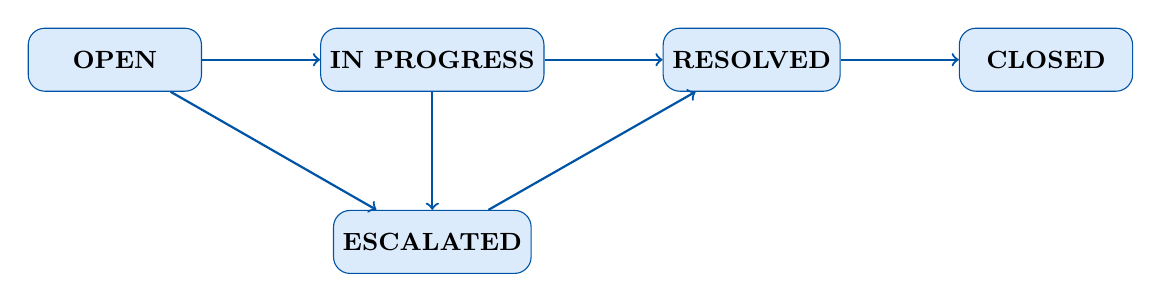
\begin{tikzpicture}[
    node distance=1.5cm,
    state/.style={rectangle, rounded corners=6pt, draw=pollityblue, fill=pollitylightblue,
                  minimum width=2.2cm, minimum height=0.8cm, font=\small\bfseries, align=center},
    arrow/.style={->, thick, color=pollityblue}
]
    \node[state] (open)       {OPEN};
    \node[state, right=of open]  (inprog) {IN PROGRESS};
    \node[state, right=of inprog] (resolved) {RESOLVED};
    \node[state, right=of resolved] (closed) {CLOSED};
    \node[state, below=of inprog] (escalated) {ESCALATED};

    \draw[arrow] (open) -- (inprog);
    \draw[arrow] (inprog) -- (resolved);
    \draw[arrow] (resolved) -- (closed);
    \draw[arrow] (open) -- (escalated);
    \draw[arrow] (inprog) -- (escalated);
    \draw[arrow] (escalated) -- (resolved);
\end{tikzpicture}
\end{center}

\newpage

% =========================================================================
% SECTION 7: IMMEDIATE ACTIONS
% =========================================================================
\section{Immediate Actions: What to Do This Week}

These are the five tasks that unblock everything else. They must be done in this order.

\begin{table}[ht]
\centering
\caption{Week 1 Action Plan}
\renewcommand{\arraystretch}{1.5}
\begin{tabularx}{\textwidth}{>{\bfseries\centering\arraybackslash}p{0.6cm} X p{2.5cm} p{2cm}}
\toprule
\rowcolor{pollitylightblue}
\textbf{\#} & \textbf{Action} & \textbf{Why It Can't Wait} & \textbf{Owner} \\
\midrule
1 & Read the Jan-Sunwai system prompt PDF in full & Defines exact NLP classification logic and conversation flows before any code is written & Piyush \\
\midrule
2 & Read the Application Questions PDF & May contain accelerator/investor constraints that shape build decisions & Manav + Piyush \\
\midrule
3 & Scaffold the full repository structure (this document) & Unblocks any contractor or co-builder from starting immediately & Piyush \\
\midrule
4 & Apply for Meta WhatsApp Business API access & Meta verification takes 3--10 business days; delays the entire Phase 1 if not started now & Piyush \\
\midrule
5 & Create Supabase project + design grievance DB schema & Everything in Phase 1 depends on the data model being finalised first & Piyush \\
\bottomrule
\end{tabularx}
\end{table}

\subsection{Pre-Seed Budget Allocation (Technical)}

Of the \$55K product development budget, the recommended technical spend:

\begin{table}[ht]
\centering
\caption{Technical Budget Breakdown}
\renewcommand{\arraystretch}{1.3}
\begin{tabularx}{\textwidth}{X p{2cm} p{4cm}}
\toprule
\rowcolor{pollitylightblue}
\textbf{Item} & \textbf{Budget} & \textbf{Notes} \\
\midrule
AWS Mumbai (EC2/ECS + RDS + ElastiCache + ALB) & \$12,000 & 12 months at approx.\ \textit{Rs.}1,000/mo infra \\
Anthropic (Claude API) credits                 & \$6,000  & Classification volume for 50 beta users + dev \\
WhatsApp Business API (Meta)                   & \$3,000  & Message volume during beta \\
Supabase Pro tier                              & \$300    & 12 months, \$25/mo \\
Sentry + PostHog                               & \$600    & 12 months \\
Domain + SSL + misc SaaS tools                 & \$500    & GitHub Teams, email, etc. \\
Frontend/backend contractor (6 weeks)          & \$20,000 & Senior full-stack contractor, Phase 1 sprint support \\
NLP contractor (4 weeks)                       & \$8,000  & Hindi/Marathi classification fine-tuning \\
Security audit                                 & \$4,600  & Phase 3 pentest \\
\midrule
\textbf{Total}                                 & \textbf{\$55,000} & \\
\bottomrule
\end{tabularx}
\end{table}

\newpage

% =========================================================================
% SECTION 8: RISKS
% =========================================================================
\section{Technical Risks \& Mitigations}

\begin{table}[ht]
\centering
\caption{Technical Risk Register}
\renewcommand{\arraystretch}{1.4}
\begin{tabularx}{\textwidth}{X p{1.8cm} p{1.8cm} X}
\toprule
\rowcolor{pollitylightblue}
\textbf{Risk} & \textbf{Probability} & \textbf{Impact} & \textbf{Mitigation} \\
\midrule
Meta WhatsApp API approval delayed & Medium & High & Apply immediately; use Twilio WhatsApp sandbox as fallback for dev \\
Claude API classification accuracy low for informal Hinglish & Medium & High & Human-in-the-loop review queue for low-confidence classifications in v1 \\
Supabase outage / data loss & Low & Critical & Daily automated backups to S3 Mumbai; multi-AZ RDS fallback plan \\
Multi-tenant data isolation breach & Low & Critical & Supabase RLS policies + integration tests that verify cross-tenant queries return empty \\
Contractor delivery delay & Medium & Medium & All work broken into 2-week sprint milestones with code review checkpoints \\
DPDP Act compliance gap & Medium & High & Engage legal counsel in Phase 3; conservative data retention defaults (90 days) \\
Redis queue overflow on high grievance volume & Low & Medium & Dead-letter queue + monitoring alert at 80\% queue depth \\
\bottomrule
\end{tabularx}
\end{table}

\vfill

\begin{center}
    {\color{midgray}\rule{0.5\linewidth}{0.5pt}}\\[0.3cm]
    {\small\itshape Pollity --- Building India's Last Mile of Digital Governance}\\
    {\small pollity.in \quad $\cdot$ \quad hello@pollity.in \quad $\cdot$ \quad \textcopyright\ 2026 Pollity}
\end{center}

\end{document}
